
\chapter{\enginline{4.} ಯೋಗಚಿಕಿತ್ಸಾ ವಿಧಾನ}

ಇತ್ತೀಚಿನ ದಿನಗಳಲ್ಲಿ ಜಗತ್ತಿನ ಜನರಲ್ಲೆಲ್ಲ ಮಾನಸಿಕ ಒತ್ತಡದಿಂದಾಗಿ ಒದಗಿ ಬರುವು ಕಾವು, ನೋವು, ಸಾವುಗಳು ಮಿತಿಮೀರಿದ ವೇಗದಲ್ಲಿ ಹೆಚ್ಚಾಗುತ್ತಿವೆ. ಅದರಲ್ಲೂ ಬುದ್ಧಿಜೀವಿಗಳಾದ ನಗರವಾಸಿಗಳನ್ನು ಇನ್ನಷ್ಟು ವಿಶೇಷವಾಗಿ ಈ ರೋಗಗಳು ಕಾಡುತ್ತಿವೆ. ಆದಕಾರಣ ಪ್ರತಿಯೊದು ತರದ ಯೋಗಾಭ್ಯಾಸದಿಂದಲೂ ಆ ಕಾಯಿಲೆಗಳನ್ನು ಹೇಗೆ ಗುಣಪಡಿಸಲು ಸಾಧ್ಯವಿದೆ—ಎಂಬುದನ್ನು ಚಿಕಿತ್ಸಾದೃಷ್ಟಿ ಯಿಂದ ಆಳವಾಗಿ ಅಧ್ಯಯನ ಮಾಡುವುದು ಇಂದಿಗೆ ಬಹಳ ಆಗತ್ಯವಾಗಿದೆ. ಆ ತರದ ಅಧ್ಯಯನ ನಡೆದು ಯೋಗಾಭ್ಯಾಸದ ಉತ್ತಮ ಪ್ರತಿಕ್ರಿಯೆ ಸ್ಥಾಪಿತಗೊಳ್ಳ ಬೇಕು. ಆಗ ಯೋಗ ಚಿಕಿತ್ಸಾವಿಧಾನವನ್ನು ತಲೆದೋರಿದ ಕಾಯಿಲೆಗಳನ್ನು ಗುಣ ಪಡಿಸಲಿಕ್ಕೂ, ಆ ಕಾಯಿಲೆಗಳು ಬಾರದಂತೆ ಮಾಡುವುದಕ್ಕೂ ಬಳಸಬಹುದಾಗಿದೆ. ಈ ವಿಷಯದಲ್ಲಿ ಮೊದಲ ಅಧ್ಯಯನ ನಡೆಸಿದ ಡಾ~। ಕುವಲಯಾನಂದ ಮತ್ತು ಡಾ~। ವೇಣೆಕರ್ ಅವರು ಹೀಗೆ ಹೇಳುತ್ತಾರೆ: "ಯೋಗ ಚಿಕಿತ್ಸಾ ವಿಧಾನಕ್ಕೆ ಇರುವ ನಿಜವಾದ ಸ್ಥಾನವೆಂದರೆ ಮನೋದೈಹಿಕ ಕಾಯಿಲೆಗಳು. ಅವಕ್ಕೆ ಯೋಗ ಚಿಕಿತ್ಸೆ ನಡೆಸಿ ವಿಶಿಷ್ಟ ಗುಣಪಡಿಸಲು ಸಾಧ್ಯವಿದೆ. ಆದರೆ ಬರೇ ಯೋಗಾ ಚಿಕಿತ್ಸಾ ವಿಧಾನದಿಂದ ಉಲ್ಬಣಾವಸ್ಥೆಗೆ ಬಂದ ರೋಗಿಗಳನ್ನು ಗುಣಪಡಿಸಲು ಸಾಧ್ಯವಾಗ ಲಾರದು. ಸಂಕ್ರಾಮಿಕ ರೋಗದ ಮಟ್ಟಕ್ಕೆ ಬಂದಾಗ ನಿವಾರಿಸಲಿಕ್ಕೂ ಸಾಧ್ಯ ವಾಗಲಾರದು. ಆದರೆ ಮೊದಲೇ ಹೇಳಿದಂತೆ ಯೋಗಾಭ್ಯಾಸದಿಂದ ದೈಹಿಕ ಮಾನಸಿಕ ಸಾಮರ್ಥ್ಯ ಹೆಚ್ಚಿ ಪ್ರತಿರೋಧಕ ಶಕ್ತಿ ಬೆಳೆದುಬರುವುದರಿಂದ ಅಂತಹ ರೋಗ ಬಾರದಂತೆ ತಡೆಗಟ್ಟಲು ಸಾಧ್ಯವಾಗಬಹುದು. ಅಷ್ಟೇ ಅಲ್ಲದೆ ತಕ್ಕ ಔಷಧೋಪಚಾರ ನಡೆದ ನಂತರ ರೋಗಿ, ತನ್ನ ಹಿಂದಿನ ಶಕ್ತಿಯನ್ನು ಪಡೆದು ಪುನರ್ಜೀವನ ನಡೆಸುತ್ತ ಬರುವಲ್ಲಿಯೂ ಯೋಗಾಭ್ಯಾಸ ಸಹಾಯಕವಾಗ ಬಹುದು. ಇವೆಲ್ಲದಕ್ಕೂ ಮುಖ್ಯವಾಗಿ, ವೈದ್ಯ ಹಾಗೂ ರೋಗಿಯ ಪರಸ್ಪರ ಸಹಕಾರ ಸಹಾನುಭೂತಿಗಳು ಅವಶ್ಯ ಬೇಕಾಗುತ್ತವೆ."

ಈ ವಿಚಾರದಲ್ಲಿ ಗಾಢವಾದ ಅಧ್ಯಯನ ನಡೆಸಿದ, ಮೇಲೆ ಹೇಳಿದ ಇಬ್ಬರು ತಜ್ಞರು ಹಾಗೂ ಇನ್ನಿತರ ಕಾರ್ಯಕರ್ತರು ಇಷ್ಟೆಲ್ಲ ಪ್ರಕಟಿಸಿದ್ದರೂ ಸಹ, ಯಾವ ಯಾವ ಯೋಗಾಭ್ಯಾಸ ನಡೆಸಿದರೆ ಏನೆಲ್ಲ ದೈಹಿಕ ಮಾನಸಿಕ ಬದಲಾವಣೆ ಗಳುಂಟಾಗುತ್ತವೆ ಎಂಬ ವಿಚಾರದಲ್ಲಿ ನಿಖರವಾದ ಅಧ್ಯಯನ ಸಾಕಷ್ಟು ನಡೆ ದಂತಿಲ್ಲ. ಹಾಗಾದ ಕಾರಣ ಯೌಗಿಕ ಚಿಕಿತ್ಸಾಕ್ರಮವನ್ನು ಒತ್ತಡದ ಕಾಯಿಲೆ ಗೊಳಗಾದವರ ಮೇಲೆ ನಡೆಸುವ ಮೊದಲು, ನಿರ್ದಿಷ್ಟ ಯೋಗಾಭ್ಯಾಸವು ಸ್ವಸ್ಥ ಮಾನವರ ಮೇಲೆ ಯಾವ ಪರಿಣಾಮವನ್ನುಂಟುಮಾಡುತ್ತದೆ—ಎಂಬುದನ್ನು ಪರೀಕ್ಷಿಸಿ ನೋಡಬೇಕು.

ಹೊಸದಾಗಿ ಆವಿಷ್ಕಾರ ಮಾಡಲಾದ ಔಷಧಿಯನ್ನು ರೋಗಿಗಳ ಮೇಲೆ ಪರೀಕ್ಷಿಸಿ ನೋಡುವ ಮೊದಲು ಆರೋಗ್ಯವಂತರಿಗೆ ಕೊಟ್ಟು ಅದರಿಂದ ಏನಾಗುವು ದೆಂದು ಅಧ್ಯಯನಗೈದು ನೋಡುವುದಿದೆ ತಾನೆ? ಅದೇ ರೀತಿ ಈ ಯೌಗಿಕ ಚಿಕಿತ್ಸಾ ವಿಧಾನದಲ್ಲೂ ಮಾಡುವುದೊಳ್ಳೇದು. ಅಂತಹ ಅಧ್ಯಯನದ ನಂತರ ಈ ಯೋಗಚಿಕಿತ್ಸೆ ನಡೆಸುವುದುತ್ತಮ.

ಅದಕ್ಕೋಸ್ಕರ ಹಲವಾರು ಸಮರ್ಥ ವಿದ್ಯಾರ್ಥಿಗಳ ತಂಡವನ್ನು ಆಯ್ಕೆ ಮಾಡಿಕೊಂಡು ನಿರ್ದಿಷ್ಟ ಯೋಗಾಭ್ಯಾಸಕ್ರಮಗಳಿಗೆ ಅವರನ್ನೊಳಪಡಿಸಿದೆವು. ನಂತರ ಅವರ ದೇಹ ಮನಸ್ಸುಗಳ ಪರಿಸ್ಥಿತಿಯನ್ನು ವೈಜ್ಞಾನಿಕವಾಗಿ ಅಧ್ಯಯನ ಗೈದೆವು. ಆ ಫಲಿತಾಂಶಗಳನ್ನು ನಾವು ಈಗಾಗಲೇ ಪ್ರಕಟಿಸಿದ್ದೇವೆ. ಹಾಗೆ ಪ್ರಯೋಜನಕಾರಿ ಪರಿಣಾಮಗಳು ತೋರಿಬಂದುದರಿಂದ ನಂತರ ಚಿಕಿತ್ಸಕದೃಷ್ಟಿ ಯಿಂದ ಆ ಯೋಗಾಭ್ಯಾಸಗಳ ಪರಿಣಾಮಗಳನ್ನು ಅಧ್ಯಯನ ಮಾಡತೊಡಗಿದೆವು.

ಅದಕ್ಕಾಗಿ, ಒತ್ತಡದ ಕಾಯಿಲೆಗಳಿಗೆ ಒಳಗಾದವರನ್ನು ವಿಸ್ತಾರವಾದ ಪರೀಕ್ಷೆ ಗಳಿಗೊಳಪಡಿಸಿದೆವು. ಅವರ ಜೀವನಚರಿತ್ರೆ, ಪ್ರಯೋಗಶಾಲೆಗಳಲ್ಲಿ ನಾನಾ ತರದ ಪರೀಕ್ಷೆ, ಎಕ್ಸ್ರೇ ಪರೀಕ್ಷೆ—ಮೊದಲಾದುವನ್ನೆಲ್ಲ ನಡೆಸಿ ಸರಿಯಾದ ಕಾಯಿಲೆ ಯಾವುದು ಎಂಬುದನ್ನು ನಿರ್ದಿಷ್ಟವಾಗಿ ತಿಳಿದುಕೊಂಡೆವು. ಹಾಗೆ ಒಮ್ಮೆ ರೋಗನಿದಾನ ಗೊತ್ತಾದಮೇಲೆ ಅವರಿಗೆ ಮೊದಲು ಮಾಮೂಲಿ ಚಿಕಿತ್ಸಾ ಕ್ರಮವನ್ನು ನಡೆಸಲಾಯಿತು. ಹಾಗೆ ನಿಶ್ಚಿತಚಿಕಿತ್ಸಾವಿಧಾನವನ್ನು ನಿರ್ದಿಷ್ಟ ಕಾಲದ ತನಕ ನಡೆಸಿಯೂ ಹೆಚ್ಚಿನ ಪ್ರಯೋಜನ ದೊರಕದ ಸಂದರ್ಭದಲ್ಲಿ ಅಂತಹ ರೋಗಿಯನ್ನು 'ಯೋಗಾಧ್ಯಯನ ಕೇಂದ್ರ'ಕ್ಕೆ ಕಳಿಸಿಕೊಡಲಾಯಿತು. ಅಲ್ಲಿ ಔಷಧೋಪಚಾರದೊಂದಿಗೆ ಯೋಗಚಿಕಿತ್ಸಾ ವಿಧಾನವನ್ನು ಸಹ ನಡೆಸಲು ಸಾಧ್ಯ ವಾಗಬಹುದೇ—ಎಂದು ಪರೀಕ್ಷಿಸಿ ನೋಡಲಾಯಿತು. ಅಂತಹ ಪ್ರಾರಂಭಿಕ ಪರೀಕ್ಷೆಯ ನಂತರ ಅವರನ್ನು ಯೋಗಾಧ್ಯಯನ ಸಂಸ್ಥೆಗೆ ಆಗಾಗ್ಗೆ ಬರಹೇಳಿ ಕೆಲವೆಲ್ಲ ಸರಿಹೊಂದುವ ಯೌಗಿಕ ಚಿಕಿತ್ಸೆಯನ್ನು ಕಲಿಸಿಕೊಡಲಾಯಿತು. ಆ ನಂತರ ಸಹ ನಿಶ್ಚಿತ ದಿನಗಳಲ್ಲಿ ಆಗಾಗ ಅವರನ್ನು ಬರಹೇಳಿ ಯೋಗಚಿಕಿತ್ಸೆಯ ಪರಿಣಾಮ ವನ್ನು ಪರೀಕ್ಷಿಸಿ ಅಧ್ಯಯನ ಮಾಡಲಾಯಿತು.

ಅಂತಹ ಚಿಕಿತ್ಸೆ, ಪರೀಕ್ಷೆಗಳ ಪರಿಣಾಮವಾಗಿ ಮಾನಸಿಕ ಒತ್ತಡದ ರೋಗ ಗಳಿಗೊಳಗಾದವರು ಕ್ರಮೇಣ ಸುಧಾರಿಸತೊಡಗಿದರು. ಅವರು ದೈಹಿಕವಾಗಿಯೂ, ಮಾನಸಿಕವಾಗಿಯೂ ಸಮರ್ಥರಾಗುತ್ತ ಬಂದರು. ಹಾಗೆಯೇ ಕ್ರಮೇಣ ಅವರು ಔಷಧಿಗಳನ್ನು ಕಡಿಮೆ ಮಾಡುತ್ತ ಬಂದು, ಬರಬರುತ್ತ ಔಷಧಿಗಳನ್ನು ಬಿಡತೊಡಗಿ ದರು. ಆ ನಂತರ ಬರೇ ಯೋಗಚಿಕಿತ್ಸೆಯಿಂದಲೇ ಹಿಂದಿನಂತೆ ಆರೋಗ್ಯಶೀಲರಾಗಿ ಸುಖಜೀವನ ನಡೆಸಲು ಸಮರ್ಥರಾದರು. ಅಂತಹ ಸುಧಾರಣೆ ಮಾನಸಿಕ ತೃಪ್ತಿ ಸಂತೋಷಗಳನ್ನೊದಗಿಸಿದ ಕಾರಣ ಅವರು ಮತ್ತಷ್ಟು ಧೈರ್ಯವಂತರಾದರು. ಮೊದಲಿನ ಜೀವನಮಾರ್ಗದಲ್ಲಿ ಸಮರ್ಥರಾಗಿ ಮುಂದುವರಿಯುವಂತೆಯೂ ಆಯಿತು.

ಅಂತಹ ಪ್ರತಿಯೊಂದು ತಂಡದ ಅಧ್ಯಯನದ ಫಲಿತಾಂಶ ಈ ಕೆಳಗಿನಂತಿದೆ:

\textbf{ಥೈರೋಡ್ ಗ್ರಂಥಿಯ ನಂಜು} \enginline{(Thyrotoxicosis)}: ಈ ರೋಗ ಗ್ರಸ್ತರಾದ ಮೂವತ್ತು ಜನರಲ್ಲಿ ಎಂಟು ಮಂದಿ ನಿರ್ದಿಷ್ಟ ಯೋಗಾಭ್ಯಾಸ ಗಳಿಂದಾಗಿ ಸಂಪೂರ್ಣ ಸ್ವಸ್ಥರಾಗಿ ಈಗ ಯೋಗಾಭ್ಯಾಸವನ್ನು ಮಾತ್ರ ಮುಂದು ವರಿಸಿಕೊಂಡು ಹೋಗುತ್ತಿದ್ದಾರೆ. ಉಳಿದ \enginline{22} ಮಂದಿ ಯೋಗಾಸನಗಳೊಂದಿಗೆ ಅದಕ್ಕಿರುವ ಔಷಧಿಗಳಾದ \enginline{Antithyroid drugs (Beta Adrenegic Blockers and Tranquilisers)} ಗಳನ್ನು ಸೇವಿಸಿಕೊಂಡು ಬರುತ್ತಿದ್ದಾರೆ. ಇವರ ದೇಹಸ್ಥಿತಿ ಸುಧಾರಿಸತೊಡಗಿದ್ದರಿಂದ ಇವರು ಕ್ರಮೇಣ ಔಷಧಿ ಪ್ರಮಾಣವನ್ನು ಕಡಿಮೆ ಮಾಡಿಕೊಂಡು ಬರುತ್ತಿದ್ದಾರೆ. ಕಾಲಕ್ರಮೇಣ ಅವರನ್ನ ಸಹ ಕೇವಲ ಯೌಗಿಕ ಚಿಕಿತ್ಸೆಗೆ ಒಳಪಡಿಸಲು ಸಾಧ್ಯವಾಗಬಹುದು. ಈ ಎಲ್ಲ ರೋಗಿಗಳ ಸುಧಾರಣೆಯ ಅಂತಿಮ ಫಲಿತಾಂಶವನ್ನು ಇಷ್ಟರಲ್ಲೇ ಹೇಳುವುದು ಸ್ವಲ್ಪ ಅವಸರದ ಕಾರ್ಯವಾದೀತು.

\begin{figure}

\includegraphics{images/020.jpg}
\caption{ಚಿತ್ರ \enginline{32:} ಥೈರೋಡ್ ಕಾಯಿಲೆಗೊಳಗಾದವರಲ್ಲಿ ಯೋಗಾಭ್ಯಾಸದಿಂದ ತೋರಿಬಂದ ದೇಹದ ತೂಕ ಮತ್ತು ನಾಡೀ ಬಡಿತಗಳ ಸುಧಾರಣೆ.}
\end{figure}

ಆದರೆ ಈ ವರೆಗಿನ ನಮ್ಮ ಅಧ್ಯಯನದ ಪ್ರಕಾರ ನಿರ್ದಿಷ್ಟ ಯೋಗಾಭ್ಯಾಸ ವನ್ನು ಶ್ರದ್ಧೆಯಿಂದ ಸರಿಯಾಗಿ ನಡೆಸಿಕೊಂಡು ಬಂದವರು, ಹಾಗೂ ಈ ರೋಗ ಬಂದು ಹೆಚ್ಚು ಸಮಯ ಆಗದವರು ಯೋಗಾಭ್ಯಾಸದಿಂದ ಸ್ವಸ್ಥರಾಗಬಹುದೆಂದು ನಾವು ಹೇಳಬಹುದಾಗಿದೆ. ಅಷ್ಟೇ ಅಲ್ಲದೆ ಯೋಗಾಭ್ಯಾಸವನ್ನು ಮುಂದುವರಿಸಿ ಕೊಂಡು ಬಂದರೆ ರೋಗ ಮರುಕಳಿಸಿ ಬರುವ ಸಂಭವ ಕಡಿಮೆಯಾಗುತ್ತದೆ. ಥೈರೋಡ್ ಗ್ರಂಥಿಯ ನಂಜುರೋಗ ಮರುಕಳಿಸಿ ಬರುವುದು ಸರ್ವಸಾಮಾನ್ಯ ವಾಗಿದೆ. ಆದ್ದರಿಂದ ಯೋಗಾಭ್ಯಾಸದ ಮೂಲಕ ಇನ್ನೊಮ್ಮೆ ಆ ರೋಗ ತಾಗದಂತೆ ನೋಡಿಕೊಳ್ಳುವುದುತ್ತಮವೆಂದು ನಾವು ರೋಗಿಗಳಿಗೆ ಹಿತವಚನ ನುಡಿಯುತ್ತೇವೆ.

\begin{figure}
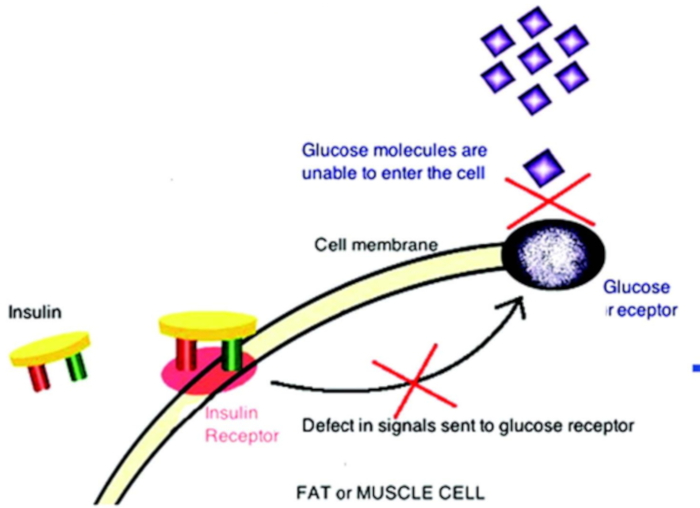
\includegraphics{images/021.jpg}
\caption{\textbf{ಚಿತ್ರ \general{\enginline{33:}} ಥೈರೋಡ್ ರೋಗಗ್ರಸ್ತ ವ್ಯಕ್ತಿಯಲ್ಲಿ ಯೋಗಾಭ್ಯಾಸದಿಂದ ತೋರಿ ಬಂದ ಸುಧಾರಣೆ.} }
\end{figure}

\textbf{ಮಿತಿಮೀರಿದ ರಕ್ತದ ಒತ್ತಡ} (Hypertension)

ನಾವು ಪ್ರತಿನಿತ್ಯ ಕಾಣುವ 'ಮಾನಸಿಕ ಅತಿ ಒತ್ತಡ' ಒಂದು ಸಾಮಾನ್ಯ ಕಾಯಿಲೆಯಾಗಿದೆ. ಇದು ಜಗತ್ತಿನಾದ್ಯಂತ ವಿಶಾಲವಾಗಿ ಹಾಗೂ ವೇಗವಾಗಿ ಹರಡುತ್ತಿರುವ ಕಾಯಿಲೆಯೂ ಆಗಿದೆ. ಅದರಲ್ಲೂ ವಿಶೇಷವಾಗಿ ನಾಗರಿಕತೆ ಬಹಳವಾಗಿ ಬೆಳೆ ದಿರುವ ಪಾಶ್ಚಾತ್ಯ ದೇಶಗಳಲ್ಲಿ ಮಿತಿಮೀರಿ ಹೆಚ್ಚುತ್ತಲೂ ಇದೆ. ಇದಕ್ಕೆ ಚಿಕಿತ್ಸಾ ರೂಪದಲ್ಲಿರುವ \enginline{Methyl Dropa} ಮೊದಲಾದ ಔಷಧಿಗಳಿಂದ ಮಾತ್ರ ಇದನ್ನು ತಡೆಗಟ್ಟಲು ಸಾಧ್ಯವಾಗುತ್ತಿಲ್ಲ. ಆದ್ದರಿಂದ ಯೋಗಾಭ್ಯಾಸ ಮುಂತಾದ ಔಷಧೇತರ ಚಿಕಿತ್ಸಾ ವಿಧಾನಕ್ಕೂ ಸ್ಥಾನ ದೊರಕುವಂತಾಗಿದೆ.

\begin{figure}
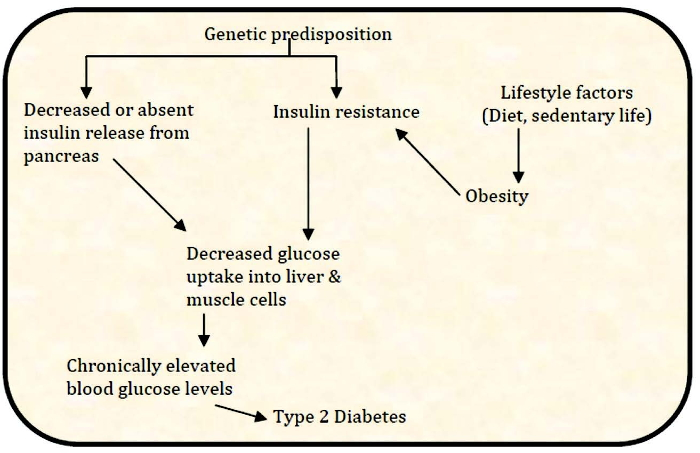
\includegraphics{images/022.jpg}
\caption{\textbf{ಚಿತ್ರ \general{\enginline{34:}} ಯೋಗಾಭ್ಯಾಸ ಮತ್ತು ಔಷಧೋಪಚಾರ ನಡೆಸಿ ರೋಗಿಗಳ, ರಕ್ತದ ಒತ್ತಡ ಕಡಿಮೆಯಾಗುತ್ತ ಬಂದುದನ್ನು ಕಾಣಬಹುದು.} }
\end{figure}

ಈ ಕಾಯಿಲೆಗೊಳಗಾದವರನ್ನು ಪರೀಕ್ಷಿಸಿ ಅವರ \enginline{Neuro–humoral} ಬದ ಲಾವಣೆಗಳನ್ನು ಅಧ್ಯಯನ ಮಾಡಿ ನೋಡಿದಾಗ ಅವರ ರಕ್ತದಲ್ಲಿ ಶಿಥಿಲವಾಗಿ ಹಾಗೂ ಹೆಚ್ಚಾಗಿ ಸ್ರವಿಸುತ್ತಿರುವ \enginline{Catecholamine} ಎಂಬುದು ಬಹು ದೊಡ್ಡ ವಿಶೇಷಾಂಶವಾಗಿದೆ. ಅದಕ್ಕಾಗಿ ಸುಲಭಸಾಧ್ಯವಾದ \enginline{30} ನಿಮಿಷಗಳ ಶವಾಸನ ನಡೆಸುವಂತೆ ಸಲಹೆ ಇತ್ತಾಗ ಈ ರೋಗಗ್ರಸ್ತರಲ್ಲಿ ಆಶಾದಾಯಕ ಫಲಿತಾಂಶ ತೋರಿಬಂತು. ಶವಾಸನ ರಕ್ತದ \enginline{Plasma Catecholamine} ನ್ನು ಕಡಿಮೆ ಗೈಯುತ್ತದೆ ಎಂಬುದನ್ನು ನಾವು ಈಗಾಗಲೇ ಕಂಡುಕೊಂಡಿದ್ದೇವೆ. ಕ್ರಮೇಣ ಇನ್ನೂ ಕೆಲವು ಆಸನಾಭ್ಯಾಸಗಳನ್ನು ಮತ್ತು ಪ್ರಾಣಾಯಾಮ ವಿಧಾನಗಳನ್ನು ನಡೆಸಿಕೊಂಡು ಬರಲು ಸಲಹೆ ಕೊಟ್ಟೆವು. ಹೆಚ್ಚಿನವರಲ್ಲಿ ಸಮಗ್ರ ಮಾನಸಿಕ ಪರಿಸ್ಥಿತಿ ಉತ್ತಮ ತರದಲ್ಲಿ ಸುಧಾರಣೆಗೊಂಡುದೂ ತೋರಿಬಂತು. ಮತ್ತೆ ಕೆಲವರಿಗೆ ಔಷಧೋಪ ಚಾರದೊಂದಿಗೆ ಯೋಗಾಭ್ಯಾಸವನ್ನು ನಡೆಸಲೂ ಸಲಹೆ ಇತ್ತೆವು. ಆಗ ಸುಧಾರಣೆ ಬೇಗನೆ ತೋರಿಬಂತು. ಅಂಥವರಿಗೆ ಸ್ವಲ್ಪ ಸಮಯದ ನಂತರ ಬರೇ ಯೋಗಾಭ್ಯಾಸ ಮಾಡಿಕೊಂಡು ಮುಂದಿನ ಜೀವನ ರೋಗಬಾಧೆ ಇಲ್ಲದೆ ನಡೆಸಿಕೊಂಡು ಬರಲೂ ಸಲಹೆ ಕೊಡಲಾಯಿತು.

ಯೋಗಾಭ್ಯಾಸದಿಂದ ಗುಣಮುಖರಾದವರ ಮೂತ್ರ ಪರೀಕ್ಷೆ ನಡೆಸಿದಾಗ \enginline{Adrenaline} ಮತ್ತು \enginline{Nonadrenaline} ಸ್ರಾವವು ಕಡಿಮೆಯಾಗಿ ಸಾಮಾನ್ಯ ಸ್ಥಿತಿಗೆ ಬಂದುದು ತೋರಿಬಂತು. ಅದರಲ್ಲೂ ಬಹಳ ಹೆಚ್ಚಿಗಿದ್ದ \enginline{Nonadrenaline contents} ಕುಗ್ಗಿ ಸಾಮಾನ್ಯಸ್ಥಿತಿಗೆ ಬಂದುದು ವಿಶೇಷವೆಂದೇ ಹೇಳಬೇಕು.

ಹೀಗೆ, ಈ ಕಾಯಿಲೆಯುನ್ನು ವಿವಿಧ ರಾಸಾಯನಿಕ ಮಿಶ್ರಣ ಕೊಡದೇನೇ ದೈಹಿಕ ಯೋಗಾಭ್ಯಾಸದಿಂದ ಹಿಡಿತಕ್ಕೆ ತರಬಹುದೆಂದು ಹೇಳಬಹುದಾಗಿದೆ. ಅಂತಹ ರಾಸಾಯನಿಕ ಔಷಧ ಪ್ರಯೋಗವಿಲ್ಲವಾದರೆ ಅಡ್ಡ ಕಾಯಿಲೆಗಳು ಬರುವ ಸಂಭವ ಇಲ್ಲ.ಅದೊಂದು ಅಭ್ಯಾಸವಾಗಿ ಅಂಟಿಕೊಳ್ಳುವ ಸಂಭವವೂ ಇಲ್ಲ.

ಆದ ಕಾರಣ, ಯೋಗಾಭ್ಯಾಸದ ಮೂಲಕ ಈ ಅತಿ ಒತ್ತಡದ ಕಾಯಿಲೆಯನ್ನು ಗುಣಪಡಿಸಬಹುದೆಂಬ ವಿಚಾರವನ್ನು ಜಗತ್ತಿನಾದ್ಯಂತ ಜನಪ್ರಿಯಗೊಳಿಸುವುದಕ್ಕೆ ತಕ್ಕ ಕಾರ್ಯಕ್ರಮ ಕೈಗೊಳ್ಳುವುದು ಉತ್ತಮವಲ್ಲವೇ?

\textbf{ಹೃನ್ನಾಳದಲ್ಲಿ ರಕ್ತಘನೀಭವನ} (Coronary Thrombosis)

ಈ ರೋಗವು ಹೆಚ್ಚಿನ ಸಂದರ್ಭಗಳಲ್ಲಿ ಹೆಚ್ಚಿದ ರಕ್ತದೊತ್ತಡ ಕಾಯಿಲೆಯ ಉಲ್ಬಣಾವಸ್ಥೆಯಾಗಿರುತ್ತದೆ. ಆ ಕಾರಣ ಗಂಟಲ ಊತದ (Angina) ಮೊದಲ ಲಕ್ಷಣ ತೋರಿಬಂದೊಡನೆ, ಮೇಲೆ ಹೇಳಿದ ಯೋಗಾಭ್ಯಾಸ ನಡೆಸಿ ಅದು ಬಾರ ದಂತೆ ಅಥವಾ ಬೆಳೆಯದಂತೆ ಮಾಡುವುದೇ ಉತ್ತಮ ಪರಿಹಾರ ಮಾರ್ಗವಾಗಿದೆ. ಆದರೆ ಇಷ್ಟರಲ್ಲೇ ಈ ರೋಗ ಬಂದಾಗಿದ್ದರೆ, ಯೋಗಾಭ್ಯಾಸದಿಂದ ಹೆಚ್ಚಿನ ಪ್ರಯೋಜನ ತೋರಿಬರಲಾರದು. ಆದರೆ ಕ್ರಮಬದ್ಧವಾದ ಶವಾಸನಾಭ್ಯಾಸವು ಈ ರೋಗ ಇನ್ನಷ್ಟು ಬೆಳೆದು ಬರದಂತೆ ಮಾಡಲು ಸಹಾಯಕವಾಗಬಹುದು.

ಈ ರೋಗಗ್ರಸ್ತರ ರಕ್ತಪರೀಕ್ಷೆಗೈದಾಗ ಅದರಲ್ಲಿ \enginline{Catecholamine} ಗಣನೀಯ ಮಟ್ಟದಲ್ಲಿ ಹೆಚ್ಚಿದ್ದೂ, \enginline{Prostoglandines} ಕುಂದಿಬಂದದ್ದೂ ತೋರಿಬಂತು. ಅಂತಹ \enginline{Neurohumoral} ಬದಲಾವಣೆಗಳು ಅತಿಯಾದ ರಕ್ತದೊತ್ತಡ ಇರುವವರಲ್ಲೂ ಕಂಡುಬರುತ್ತದೆ. ಆದರೆ ಹೃನ್ನಾಳ ರೋಗಗ್ರಸ್ತರಲ್ಲಿ \enginline{(Coronary Diseases)} ಈ ಏರಿಳಿತಿಗಳು ಮಿತಿಮೀರಿ ಕಂಡುಬರುತ್ತದೆ. ಆದ ಕಾರಣ ಅತಿ ರಕ್ತದೊತ್ತಡದ ಕಾಯಿಲೆಯವರಿಗೆ ಸಲಹೆಗೈಯಲಾದ ಶವಾಸನವನ್ನು ಇವರಿಗೂ ಹೇಳಿಕೊಡುವುದು ಸಮಂಜಸವಾಗುತ್ತದೆ. ಈ ವಿಚಾರದಲ್ಲಿ ನಮ್ಮ ಅನುಭವ ಪರಿಮಿತವಾದುದು. ಏಕೆಂದರೆ ಇದು ಭಯಂಕರ ಕಾಯಿಲೆಯಾದ್ದರಿಂದ ಈ ರೋಗಿಗಳನ್ನು ಯೋಗಾಭ್ಯಾಸದಿಂದ ಮಾತ್ರ ಗುಣಪಡಿಸಲು ಪ್ರಯತ್ನಿಸುವ ಸಾಹಸಕಾರ್ಯ ತೆಗೆದುಕೊಳ್ಳಬಾರದೆಂದು ನಿಶ್ಚಯಿಸಿದೆವು. ಔಷಧೋಪಚಾರ ದೊಂದಿಗೆ ಅದಕ್ಕೆ ಪೂರಕವಾಗಿ ಮಾತ್ರ ಕೆಲಮಟ್ಟಿನ ಯೋಗೋಪಚಾರವನ್ನು ನಡೆಸಿ, ಈ ರೋಗ ಇನ್ನಷ್ಟು ಹೆಚ್ಚದಂತೆ ಮಾಡಬಹುದೆಂದು ಸೂಚಿಸಿದೆವು. ಇದಲ್ಲದೆ \enginline{Cardiac Neurosis} ಕಾಯಿಲೆಯಲ್ಲಿ ಸಹ, ಅದು ಮೊದಲ ಹಂತ ದಲ್ಲಿದ್ದಾಗ ಈ ಯೋಗೋಪಚಾರವು ಪ್ರಯೋಜನಕಾರಿ ಎಂಬುದನ್ನು ಕಂಡು ಕೊಂಡೆವು.

\textbf{ಬಹುಕಾಲದ ಜೀರ್ಣಾಂಗ ವ್ರಣ} \enginline{(Chronic Peptic Ulcer)} ಈ ರೋಗ ಬಂದವರ ರಕ್ತದಲ್ಲಿ \enginline{Acetylcholine} ಮತ್ತು \enginline{Histomine} ಅಂಶ ಬಹಳ ಹೆಚ್ಚಾಗಿರುವುದನ್ನು ಕಾಣಬಹುದು. ಅಷ್ಟೇ ಅಲ್ಲದೆ \enginline{Plasma cortisol} ಸಹ ಬಹಳ ಹೆಚ್ಚಿರುವುದರಿಂದ ಹೆಚ್ಚಿನ ಒತ್ತಡದ ಪರಿಸ್ಥಿತಿಯೂ ಇರುತ್ತದೆ. ಆದರೆ ಈ ವಿಚಾರದಲ್ಲಿ ನಮ್ಮ ಅನುಭವದ ಪ್ರಕಾರ ಯೋಗಾಭ್ಯಾಸದಿಂದ ಹೆಚ್ಚಿನ ಪ್ರಯೋಜನ ತೋರಿಬರಲಿಲ್ಲ. ಆದರೆ ರೋಗಾರಂಭದೆಸೆಯಲ್ಲಿ ಜಠರ ವಾಯು ದೋಷ \enginline{(Functional Gastric Disorders)} ಇರುವಾಗ, ಯೋಗಾಭ್ಯಾಸ ದಿಂದ ತುಂಬಾ ಪ್ರಯೋಜನ ಉಂಟಾದುದನ್ನು ಕಂಡುಕೊಂಡಿದ್ದೇವೆ. ಇದರ ಬದಲಾಗಿ ಆಯುರ್ವೇದೀಯ ಔಷಧಿಯಾದ ಆಮಲಕಿ(ನೆಲ್ಲಿಕಾಯಿ)ಯ ಔಷಧೋಪ ಚಾರದಿಂದ ತುಂಬ ಪ್ರಯೋಜನ ದೊರಕುತ್ತದೆ. ಗುಣ ಹೊಂದಿದ \enginline{Peptic Ulcer} ಕಾಯಿಲೆಯ ಆಯ್ದ \enginline{68} ರೋಗಿಗಳ ಚರಿತ್ರೆ ನಮ್ಮಲ್ಲಿದೆ. ಈ ಔಷಧಿಯಿಂದಾಗಿ ಅವರ ರಕ್ತದ \enginline{Neurohumoral contents} ಕಡಿಮೆಯಾಗುತ್ತ ಬಂದು \enginline{Acid secretion} ಸಾಮಾನ್ಯ ಮಟ್ಟಕ್ಕೆ ಬರಲಾರಂಭಿಸಿದ್ದನ್ನು ನಾವು ಕಂಡುಕೊಂಡಿದ್ದೇವೆ.

\textbf{ದೊಡ್ಡ ಕರುಳಿನ ವ್ರಣ} \enginline{(Ulcerative Colities)}

ಈ ರೋಗಗ್ರಸ್ತರನ್ನು ಪರೀಕ್ಷಿಸಿ ನೋಡಿದರೆ ಅವರ ರಕ್ತದಲ್ಲಿ \enginline{Acetylcholine} ಮತ್ತು \enginline{Histamine} ಅಂಶಗಳು ವಿಶೇಷವಾಗಿ ಹೆಚ್ಚಗಿರುತ್ತವೆ. ಈ ಹೆಚ್ಚಳ ಬೇರೆಬೇರೆ ಮಟ್ಟದಲ್ಲಿ ರೋಗಗ್ರಸ್ತರಾದ, ಲೋಳೆ ಸ್ರವಿಸುವ ಕರುಳಿನ ರೋಗ್ರ ಸ್ತರಲ್ಲಿಯೂ \enginline{(Mucus Colitis),} ವ್ರಣ ತುಂಬಿದ ಕರುಳುರೋಗ ಉಳ್ಳವ ರಲ್ಲಿಯೂ ಕಂಡುಬಂದಿದೆ. ಈ ಎರಡೂ ತರದ ರೋಗ ಪೀಡಿತರಾದವರಿಗೆ ತಕ್ಕ ಔಷಧೋಪಚಾರದೊಂದಿಗೆ ಕೆಲವೆಲ್ಲ ಯೋಗಾಭ್ಯಾಸಗಳನ್ನು ನಡೆಸಿಕೊಂಡು ಬಂದ ವರಲ್ಲಿ ಉತ್ತಮ ಪ್ರಯೋಜನ ತೋರಿಬಂದಿದೆ. ಅದರಲ್ಲೂ ವಿಶೇಷವಾಗಿ ಕರುಳಿನ ಕಾಯಿಲೆಗಳ ಆರಂಭಾವಸ್ಥೆಯಲ್ಲಿ ಬಹು ಬೇಗನೆ ಗುಣಾಂಶ ತೋರಿ ಬಂದಿದೆ.

\textbf{ಕಳವಳಮಯ ನರದೌರ್ಬಲ್ಯ} \enginline{(Anxiety Neurosis)}

ಈ ಕಾಯಿಲೆಗೆ ಗುರಿಯಾದವರು ನಿಷ್ಕಾರಣ ಕಳವಳ, ಮಾನಸಿಕ ತುಮುಲಗಳಿಂದ ಸದಾ ನರಳುತ್ತಿರುತ್ತಾರೆ. ಬಹಳವಾದ ಮಾನಸಿಕ ಕೆಲಸದ ಒತ್ತಡಕ್ಕೆ ಗುರಿಯಾಗಿ ತವಕಪಡುತ್ತಿದ್ದವರನ್ನು ಈ ಕಾಯಿಲೆ ವಿಶೇಷವಾಗಿ ಕಾಡುತ್ತದೆ. ಅಂಥವರು ನಿಷ್ಕಾರಣ ಭಯಸಂದೇಹಗಳಿಗೊಳಗಾಗಿ ಶೀಘ್ರಕೋಪಿಗಳಾಗಿ ಇರುತ್ತಾರೆ. ನಿದ್ರೆ ಬಾರದೆ, ಕೆಲವೇಳೆ ಮಿತಿಮೀರಿದ ಎದೆಬಡಿತ ಮುಂತಾದ ತೊಂದರೆಗಳಿಗೊಳಗಾಗುತ್ತಾರೆ. ಅವರ ರಕ್ತದಲ್ಲಿ ಹೆಚ್ಚಾದ \enginline{Acetycholine} ಉಂಟಾಗಿ, ವಿಶೇಷ \enginline{Neurohumoral} ಬದಲಾವಣೆಗಳು ಕಂಡುಬರುತ್ತವೆ ಇಂಥವರಿಗೆ ಯೋಗಾಸನ, ಪ್ರಾಣಾಯಾಮ ಮತ್ತು ಧ್ಯಾನಗಳುಳ್ಳ ಸಂಯುಕ್ತಾಭ್ಯಾಸವು ಬಹುಬೇಗನೆ ಉತ್ತಮ ಪರಿಣಾಮವನ್ನುಂಟುಮಾಡುತ್ತದೆ. ಇವರು ಮೂರರಿಂದ ಆರು ತಿಂಗಳವರೆಗಿನ ಈ ಸಂಯುಕ್ತಾಭ್ಯಾಸದಿಂದ ಗುಣಮುಖರಾಗುತ್ತಾರೆ. ಅದಲ್ಲದೆ ಮೂತ್ರದಲ್ಲಿ ಹೆಚ್ಚಾಗಿದ್ದ \enginline{Urinary nonadrenaline} ಮಟ್ಟ ಸಾಮಾನ್ಯಮಟ್ಟಕ್ಕೆ ಕೆಲವೇ ದಿನಗಳಲ್ಲಿ ಬಂದು ನಿಲ್ಲುತ್ತದೆ. ಅವರ ದೈಹಿಕ ಅಥವಾ ಜೀವರಾಸಾಯನಿಕ ಸುಧಾರಣೆಗಿಂತಲೂ ಬಹುಮೊದಲೇ ಅವರ ವೈಯಕ್ತಿಕ ಮನೋಭಾವನೆಗಳ ಸುಧಾರಣೆ ಕಂಡುಬರುತ್ತದೆ. ಹೀಗೆ ದೀರ್ಘಕಾಲೀನ ಯೋಗಾಭ್ಯಾಸದಿಂದ ಈ ರೋಗವನ್ನು ಸಂಪೂರ್ಣ ಗುಣಪಡಿಸಲಾಗುತ್ತದೆ ಎಂಬುದು ನಮ್ಮ ಅಧ್ಯಯನ ದಿಂದ ತಿಳಿದುಬಂದಿದೆ. ಆದರೆ ಹಾಗೆ ನಿತ್ಯಾಭ್ಯಾಸ ಇಟ್ಟುಕೊಳ್ಳದಿದ್ದರೆ ರೋಗ ಮರುಕಳಿಸುವ ಸಂಭವವೂ ಉಂಟು.

\textbf{ಶ್ವಾಸನಾಳದ ಉಬ್ಬಸ \general{\enginline{(Bronchial Asthma)}}}

ಈ ರೋಗವನ್ನು ಸಂಪೂರ್ಣ ಗುಣಪಡಿಸುವುದಕ್ಕೆ ತಕ್ಕ ಆಧುನಿಕ ಔಷದಿ \enginline{(Modern Medicine)} ಈಗಿನ ಮಟ್ಟಿಗೆ ದೊರಕುತ್ತಿಲ್ಲ. ಹಾಗಾಗಿ ಔಷಧದಿಂದ ಗುಣಪಡಿಸಲಾಗದ ಕೆಲವು ರೋಗಿಗಳಿಗೆ ಈ ಯೋಗಚಿಕಿತ್ಸೆ ನಡೆಸಿ ತಕ್ಕಮಟ್ಟಿನ ಪ್ರಯೋಜನ ಪಡೆದಿದ್ದಾರೆ. ಈ ರೋಗಗ್ರಸ್ತರಲ್ಲಿ ಸ್ಪಷ್ಟವಾದ ದೊಡ್ಡ ನ್ಯೂನತೆ ಎಂದರೆ ರಕ್ತದಲ್ಲಿ ಹೆಚ್ಚಿನ ಮಟ್ಟದಲ್ಲಿರುವ \enginline{Histamine} ಮತ್ತು \enginline{Hista minase} ನ ಅಂಶವಾಗಿದೆ. ಅಷ್ಟೇ ಅಲ್ಲದೆ, ಮೂತ್ರವಿಸರ್ಜನೆಯಲ್ಲಿ \enginline{Adrenaline} ಮತ್ತು \enginline{Nonadrenaline} ಅಂಶ ಕಡಿಮೆಯಾಗಿರುತ್ತದೆ. \enginline{Cycli AMP} ಸಹ ತುಂಬ ಕಡಿಮೆಯಾಗಿರುತ್ತದೆ. ಆದರೆ ಯೋಗಾಭ್ಯಾಸ ಮಾಡತೊಡಗಿದ ನಂತರ ಮೂತ್ರದ \enginline{Neurohumoral contents} ನಲ್ಲಿ ಗಣನೀಯ ಬದಲಾವಣೆ ತೋರಿ ಬಂತು. \enginline{Catecholamines} ಮತ್ತು \enginline{Corticoid} ಹೆಚ್ಚಾದುದೂ ಕಂಡುಬಂತು. ಹೀಗೆ ಕಡಿಮೆ ಮಟ್ಟದಲ್ಲಿದ್ದ ಈ ಮೇಲಿನ ಅಂಶಗಳು ಯೋಗಾಭ್ಯಾಸದಿಂದ ದೇಹದಲ್ಲಿ ಹೆಚ್ಚು ಹೆಚ್ಚು ಉತ್ಪಾದನೆಯಾಗತೊಡಗಿದ್ದು ಈ ಗುಣಾಂಶ ತೋರಿ ಬರುವುದಕ್ಕೆ ಕಾರಣವಾಗಿರಬೇಕು.

\textbf{ಮಧುಮೇಹ \general{\enginline{(Diabetes Mellitus)}} }

ಈ ರೋಗವನ್ನು ಗುಣಪಡಿಸಲು ಔಷಧೋಪಚಾರದ ಜೊತೆಗೆ ಯೋಗಾಭ್ಯಾಸವನ್ನು ನಡೆಸಿಕೊಂಡು ಬಂದರೆ ತುಂಬ ಪ್ರಯೋಜನ ದೊರಕುತ್ತದೆ. ಯೋಗಾಸನದೊಂದಿಗೆ ಪ್ರಾಣಾಯಾಮವನ್ನೂ ನಡೆಸಿಕೊಂಡು ಬಂದರೆ ಕ್ರಮೇಣ ಔಷಧಿ ಸೇವನೆಯನ್ನು ಕಡಿಮೆ ಮಾಡಿಕೊಂಡು ಬರುವುದಕ್ಕೂ ಸಾಧ್ಯವಾಗುತ್ತದೆ. ಅದರಲ್ಲಿಯೂ ವಿಶೇಷ ವಾಗಿ ಮಧ್ಯವಯಸ್ಕರಲ್ಲಿ ಈ ರೋಗವು ಆರಂಭಾವಸ್ಥೆಯಲ್ಲಿರುವಾಗ ಯೋಗ ಬಹಳ ಪರಿಣಾಮಕಾರಿ. ಆದರೆ ಈ ಯೋಗಾಭ್ಯಾಸವನ್ನು ಜೀವನವಿಡೀ ನಡೆಸಿ ಕೊಂಡು ಬರಬೇಕಾಗುತ್ತದೆ. ಇಲ್ಲವಾದರೆ ರೋಗ ಮರುಕಳಿಸಲೂಬಹುದು. ರೋಗ ಬಹಳ ಬೆಳೆದುಬಂದಿದ್ದರೆ ಅಂಥವರಿಗೆ ಯೋಗಾಭ್ಯಾಸವು ಆದರ ತೀವ್ರತೆ ಯನ್ನು ಕಡಿಮೆ ಮಾಡುತ್ತದೆ. ಅದಕ್ಕೆ ಕಾರಣ ಯೋಗಾಭ್ಯಾಸ ರಕ್ತದ \enginline{Catecholamine} ಅಂಶವನ್ನು ಕುಗ್ಗಿಸಿ ರಕ್ತದ ಸಕ್ಕರೆಯ ಪ್ರಮಾಣವನ್ನು ಹಿಡಿತಕ್ಕೆ ತರುತ್ತದೆ. ಮಾನಸಿಕ ಒತ್ತಡಗಳಿಗೊಳಗಾದ ಮಧುಮೇಹಗ್ರಸ್ತರಿಗೆ ಯೋಗಾಭ್ಯಾಸ ತುಂಬ ಉಪಕಾರಿಯಾಗುತ್ತದೆ.

\textbf{ಬೆನ್ನು ಮೂಳೆಯ ವಾತರೋಗ} \enginline{(Rheumatic disorders of the Spine)}

ಈ ರೋಗ್ರಸ್ತರಿಗೆ ಯೋಗಾಸನಾಭ್ಯಾಸ ಬಹುಬೇಗ ಉತ್ತಮ ಪರಿಣಾಮ ತೋರಿ ಬರುವಂತೆ ಮಾಡುತ್ತದೆ. ಬಹುತೇಕವಾಗಿ ಈ ರೋಗಗ್ರಸ್ತರಲ್ಲಿ ಬರೇ ಔಷಧಿ ಯಿಂದ ಪ್ರಯೋಜನವಾಗುವುದಿಲ್ಲ. ಅದರಲ್ಲೂ ಪದೇಪದೇ ಬರುವ ಬೆನ್ನು ನೋವಿನ ಕಾಯಿಲೆಯಾದರೆ ಔಷಧಿಯೂ ನಾಟುವುದಿಲ್ಲ. ಆ ಸಂದರ್ಭದಲ್ಲಿ ಸರಿಯಾದ ಯೋಗಾಭ್ಯಾಸದಿಂದ ಸಂಪೂರ್ಣ ಪ್ರಯೋಜನ ತೋರಿ ಅವರು ಸುಖ ಜೀವನ ನಡೆಸುವುದಕ್ಕೆ ಸಾಧ್ಯವಾಗುತ್ತದೆ.

\textbf{ಅರ್ಬುದ ರೋಗ} \enginline{(Cancer)}

ಈ ರೋಗ ಬೆಳೆಯುವುದಕ್ಕೆ ಮಾನಸಿಕ ಒತ್ತಡ ಪ್ರಮುಖ ಪಾತ್ರ ವಹಿಸುತ್ತ ದೆಂಬುದು ವಿಭಿನ್ನ ಪ್ರಯೋಗಗಳ ಹಾಗೂ ಚಿಕಿತ್ಸಾ ವಿಧಾನಗಳ ಪರಿಶೀಲನೆಯಿಂದ ತಿಳಿದುಬರುತ್ತದೆ. ಪ್ರಾಯಶಃ ಅಂಥವರಲ್ಲಿ \enginline{Adernal Medulla} ಮತ್ತು \enginline{Cortex} ನಿಂದ ವಿಸರ್ಜಿತವಾಗುವ \enginline{Catecholamines} ಮತ್ತು \enginline{Cortisol} ಗಳು ಈ ಕಾಯಿಲೆಗೆ ಕಾರಣವಿರಬೇಕು.

ದೇಹದೊಳಗೆ ಹೆಚ್ಚಾಗಿ ಸ್ರವಿಸುವ \enginline{Cortisol,} ರೋಗಪ್ರತಿರೋಧಕ ಶಕ್ತಿ ಯನ್ನು ಕುಗ್ಗಿಸುತ್ತದೆ. ಆ ಮೂಲಕ ಅರ್ಬುದ ರೋಗದ ಬೆಳವಣಿಗೆಗೆ ಕಾರಣ ವಾಗುತ್ತದೆ. ಇದು ಈಗಾಗಲೇ ತಿಳಿದಿರುವ ವಿಚಾರವಾಗಿದೆ. ಇದರೊಂದಿಗೆ ಮಾನಸಿಕ ಒತ್ತಡದ ಕಾರಣದಿಂದಾಗಿ ಹೆಚ್ಚಿನ \enginline{Catecholamine} ವಿಸರ್ಜನೆ ಉಂಟಾದಾಗ ಈ ರೋಗವೃದ್ಧಿಗೆ ಅದೂ ಸಹಾಯಕವಾಗುತ್ತದೆ. ಅಂತಹ ಮಾನಸಿಕ ಒತ್ತಡದ ಪರಿಸ್ಥಿತಿ ಮುಂದುವರಿಯುತ್ತಾ ಇದ್ದರೆ, ಕಾರಣಾಂತರದಿಂದ ಶಕ್ತಿಹೀನ ವಾದ ಅವಯವ ಅಥವಾ ಅಂಗಾಂಶ (Tissue) ಈ ಭಯಂಕರ ರೋಗಕ್ಕೆ ಗುರಿ ಯಾಗುತ್ತದೆ. ಆ ಅವಯವ ಅಥವಾ ಅಂಗಾಂಶ ಶಕ್ತಿಹೀನವಾಗಿರುವುದಕ್ಕೆ ಆನು ವಂಶಿಕ ಕಾರಣವಿರಬಹುದು. ಇಲ್ಲವೇ ವಾತಾವರಣ ಅಥವಾ ಎಳೆತನದಿಂದಲೇ ನಡೆಸಿಕೊಂಡು ಬಂದ ಜೀವನ ವಿಧಾನವೂ ಕಾರಣವಿರಬಹುದು. ಬಹುಕಾಲ \enginline{Catecholamines} ಮೇಲ್ಮಟ್ಟದಲ್ಲಿಯೇ ಇದ್ದರೆ ಆ ಶಕ್ತಿಹೀನ ಅವಯವದಲ್ಲಿ ರಕ್ತಸಂಚಾರ ಕಡಿಮೆಯಾಗುತ್ತದೆ. ಅದರಿಂದ ಅಲ್ಲಿಯ ಅಂಗಾಂಶಕ್ಕೆ ಆಮ್ಲಜನಕ ಸಿಗದಂತಾಗುವ ಪರಿಸ್ಥಿತಿ \enginline{(Tissue anoxia)} ಒದಗಿಬರುತ್ತದೆ. ಹಾಗಾದಮೇಲೆ ಕ್ರಮೇಣ ಆ ಅಂಗಾಂಶಗಳು ವಿಚಿತ್ರರೀತಿಯಲ್ಲಿ ಬೆಳೆದುಬಂದು ಅರ್ಬುದಾಕಾರ ಪಡೆಯುತ್ತವೆ.

ಅಂತು ಇವನ್ನೆಲ್ಲ ಪರಿಶೀಲಿಸಿದಾಗ ಮಾನಸಿಕ ಒತ್ತಡ, ಅರ್ಬುದ ರೋಗ ಆರಂಭಗೊಂಡು ಬೆಳೆದುಬರುವುದಕ್ಕೆ ಒಂದು ಮುಖ್ಯ ಕಾರಣವಾಗಬಹುದು. ಅದು ಕೆಲವೇಳೆ ದೇಹದಲ್ಲಿ ಮಿತಿಮೀರಿದ ಕಾರ್ಟಿಸೊಲ್ ವಿಸರ್ಜನೆಯಿಂದಾಗಿ ರೋಗ ಪ್ರತಿರೋಧಕಶಕ್ತಿಯನ್ನು ಕುಗ್ಗಿಸುವುದರಿಂದಾಗಬಹುದು. ಅಥವಾ \enginline{Catecholamines} ನ ಹೆಚ್ಚಿನ ಪ್ರತಿಕ್ರಿಯೆಯಿಂದಾಗಿ ಉಂಟಾಗುವ \enginline{Vasoconstriction} ಮತ್ತು \enginline{Anoxio} ಗಳಿಂದ ಬೆಳೆದುಬರುವಂತಾಗಲೂ ಬಹುದು. ಆದರೆ ಅಂಗಾಂಶ ಗಳ ದುರ್ಮಾಂಸ ರೂಪದ ಕ್ಯಾನ್ಸರ್ (Sarcoma) ರೋಗಿಗಳಲ್ಲಿ ರಕ್ತ ಮತ್ತು ಅಂಗಾಂಶಗಳ \enginline{Histamine} ಮಟ್ಟ ಬಹಳ ಹೆಚ್ಚಾಗಿ ಕಂಡುಬರುವುದರಿಂದ, ಹೆಚ್ಚಿ ನಂಶ ರೋಗಪ್ರತಿರೋಧಕಶಕ್ತಿ ಇಲ್ಲದ್ದರಿಂದಾಗಿ ರೋಗ ಉಲ್ಬಣಗೊಳ್ಳುತ್ತಿರ ಬೇಕು. ಅಂತು ಮಾನಸಿಕ ತಳಮಳಗಳು ಈ ರೋಗ ಮೂಡಿಬಂದು ಹೆಚ್ಚುತ್ತ ಹೋಗುವುದಕ್ಕೆ ಕಾರಣವೆಂದು ಹೇಳಬಹುದಾಗಿದೆ. ಆದ್ದರಿಂದ ಅದಕ್ಕೆ ತಕ್ಕ ಔಷಧಿಯೊಂದಿಗೆ ಯೌಗಿಕೋಪಚಾರವನ್ನು ನಡೆಸಿದ್ದಾದರೆ ರೋಗ ಉಪಶಮನವಾಗುವು ದಕ್ಕೆ ಸಹಾಯಕವಾಗಬಹುದು.

ಸಂಕ್ಷೇಪವಾಗಿ ಹೇಳುವುದಿದ್ದರೆ ಮೇಲೆ ಹೇಳಿದ ಎಲ್ಲ ರೀತಿಯ ಮಾನಸಿಕ ಒತ್ತಡದ ಕಾಯಿಲೆಗಳಿಂದ ನಾವು ದೂರವಿರಬೇಕು. ಸಮರ್ಥ, ರಚನಾತ್ಮಕ ಕಾರ್ಯಾಸಕ್ತರಾಗಿ ಉತ್ತಮ ಜೀವನ ನಡೆಸಿಕೊಂಡು ಬರಬೇಕು. ಅದಕ್ಕಾಗಿ ಯೋಗಾಭ್ಯಾಸಗೈಯುತ್ತ ಮೇಲ್ಮಟ್ಟದ ದೈಹಿಕಮಾನಸಿಕ ಆರೋಗ್ಯ ಕಾಪಾಡಿ ಕೊಂಡು ಬರಬೇಕು. ಅಷ್ಟೇ ಅಲ್ಲದೆ, ವಿವಿಧ ಒತ್ತಡ ರೋಗಗಳಿಂದ ನರಳುತ್ತಿರು ವವರಿಗೆ ತಕ್ಕ ಔಷಧೋಪಚಾರಗಳೊಂದಿಗೆ, ಅದಕ್ಕೆ ಪೂರಕವಾಗಿ ಯೋಗಾಭ್ಯಾಸದ ಸಲಹೆಗಳನ್ನಿತ್ತು ಅವರ ಜೀವನವನ್ನು ಸುಗಮಗೊಳಿಸುವುದಕ್ಕೂ ನಾವು ಸಹಾಯ ಮಾಡಬೇಕು.

\textbf{ಜೈವಿಕ ಪುನರ್ಮಾಹಿತಿ ಮೂಲಕ ರೋಗಶಮನ ವಿಧಾನ} \enginline{(Therapeutic use of Bio–feedback Methods)
 }

ಇತ್ತೀಚಿನವರೆಗೆ, ದೇಹ ಮತ್ತು ಮನಸ್ಸಿನ ಸಂಬಂಧವನ್ನು ವೈಜ್ಞಾನಿಕ ರೀತಿಯಲ್ಲಿ ಅಳೆದು ನೋಡಲಿರುವ ಉಪಕರಣಗಳು ದೊರಕುತ್ತಿದ್ದಿಲ್ಲ. ಈ ಹಿಂದೆ, ದೈಹಿಕ ಪರಿಸ್ಥಿತಿಯಲ್ಲಿ ಬದಲಾವಣೆಯುಂಟಾದರೆ, ಅದು ಮಾನಸಿಕ ಹಾಗೂ ಭಾವನಾತ್ಮಕ ಪರಿಸ್ಥಿತಿಯನ್ನು ಬದಲಾಯಿಸುತ್ತದೆ; ಅದೇ ತರದಲ್ಲಿ ಮಾನಸಿಕ ಅಥವಾ ಭಾವನಾತ್ಮಕ ಬದಲಾವಣೆ ದೈಹಿಕ ಪರಿಸ್ಥಿತಿಯನ್ನು ವ್ಯತ್ಯಾಸಗೊಳಿಸುತ್ತದೆ ಎಂಬಂಶ ಮಾತ್ರ ಗೊತ್ತಿತ್ತು. ಇದಕ್ಕೆ ಮಿಕ್ಕಿದ, ಬಹುಮುಖ್ಯವಾದ ಆ ಸಂಬಂಧ ಯಾವ ತರದ್ದು? ಎಷ್ಟರಮಟ್ಟಿಗಿದೆ? ಎಂಬುದರ ಅರಿವು ಇದ್ದಿಲ್ಲ. ಈ ಸಂಬಂಧದ ವೈಜ್ಞಾನಿಕ ಅಧ್ಯಯನ ಮಾಡಹೊರಟ ಡಾ~। ಗ್ರೀನ್ ಮತ್ತವರ ಸಂಗಡಿಗರು ಜೈವಿಕ ಪುನರ್ಮಾಹಿತಿ ಮಾಪಕಗಳನ್ನು \enginline{(Bio feed back Meter)} ಬಳಸತೊಡಗಿ ದರು. ಆ ಮೂಲಕ ವಿವಿಧ ಸಂದರ್ಭಗಳಲ್ಲಿ ಉಂಟಾಗುವ ದೇಹದ ಉಷ್ಣಾಂಶ, ಸ್ನಾಯುಗಳ ಒತ್ತಡ, ಮಿದುಳಿನ ಅಲ್ಫಾ ಚಲನೆ—ಮುಂತಾದುವನ್ನು ನಿಖರವಾಗಿ ಪರಿಶೀಲಿಸಿ ರೆಕಾರ್ಡು ಮಾಡಿಕೊಳ್ಳುವುದಕ್ಕೆ ಸಾಧ್ಯವಾಗುವಂತಾಗಿದೆ.

ಆ ನಂತರ ದೇಹಮನಸ್ಸಂಬಂಧವನ್ನು—ಆರೋಗ್ಯದಲ್ಲಿರುವಾಗ ಮತ್ತು ಅನಾರೋಗ್ಯ ಸಂದರ್ಭದಲ್ಲಿ—ಇಷ್ಟಬಂದಾಗ ತನ್ನ ಹಿಡಿತಕ್ಕೆ ತಂದುಕೊಳ್ಳಲು ವ್ಯಕ್ತಿಯೊಬ್ಬನಿಗೆ ತರಬೇತಿ ಕೊಡಲಾಯಿತು. ಯೋಗಾಭ್ಯಾಸ, ಯೆುನ್ ಧ್ಯಾನಾಭ್ಯಾಸ ಅಥವಾ \enginline{Autogenic Training} ಮೂಲಕ ಸ್ನಾಯು ಒತ್ತಡವನ್ನು ಶಿಥಿಲ ಮಾಡಿ ಕೊಳ್ಳಲಿಕ್ಕೆ, ದೇಹದ ಉಷ್ಣಾಂಶ ಹೆಚ್ಚಿಸಿಕೊಳ್ಳಲಿಕ್ಕೆ ಅಥವಾ ಮಿದುಳಿನ ಅಲ್ಫಾ ಚಲನೆ ವೃದ್ಧಿಸಿಕೊಳ್ಳಲಿಕ್ಕೆ ಸಾಧ್ಯವಾಗುವಂತಾಯಿತು. ಹಾಗಾಗಿ ಈ ವಿಚಾರದಲ್ಲಿ ಡಾ~। ಗ್ರೀನ್ ಅಟ್​ಎಲ್ ಅವರು ಹೀಗೆ ಹೇಳುತ್ತಾರೆ: "ಮಾನವನ \enginline{50\%} ರಿಂದ \enginline{75\%} ಕಾಯಿಲೆಗಳು ಮನಃಶಾರೀರಿಕ ಕಾಯಿಲೆ \enginline{(Psycho–sometic Diseases)} ಗಳಾಗಿವೆ. ವಸ್ತುತಃ ಮನಃಶಾರೀರಿಕ ರೋಗ ಮತ್ತು ಮನಃಶಾರೀರಿಕ ಆರೋಗ್ಯ ಒಂದೇ ನಾಣ್ಯದ ಎರಡು ವಿರುದ್ಧ ಮುಖಗಳಾಗಿವೆ. ಆದಕಾರಣ ತಕ್ಕ ತರಬೇತಿ ಕೊಟ್ಟು ದೇಹ ಮನಸ್ಸಂಬಂಧಗಳ ಅರಿವುಂಟಾಗುವಂತೆ ಮಾಡಿದ್ದಾದರೆ ಅರೆತಲೆ ನೋವು ಮುಂತಾದ ಈ ಮನಃಶಾರೀರಿಕ ಕಾಯಿಲೆಗಳನ್ನು ಔಷಧೋಪ ಚಾರವಿಲ್ಲದೆ ಗುಣಪಡಿಸಲು ಸಾಧ್ಯವಿದೆ" ಎಂದು ಹೇಳಿದ್ದಾರೆ. ಮುಂದುವರಿದು ಹೀಗೂ ಅವರು ಹೇಳಿದ್ದಾರೆ:—'ಮನಃಶಾರೀರಿಕ ರೋಗವಿಲ್ಲದ ಸ್ಥಿತಿಯೇ ಮನಃ ಶಾರೀರಿಕ ಆರೋಗ್ಯ. ಈ ತತ್ವವನ್ನು ಸರಿಯಾಗಿ ಅರ್ಥಮಾಡಿಕೊಂಡರೆ, ಮಾನಸಿಕ ಗೊಂದಲ ದಲ್ಲೂ ನಮ್ಮನ್ನು ನಾವು ಹಿಡಿತಕ್ಕೆ ತಂದುಕೊಳ್ಳಲಿಕ್ಕೆ ಸಾಧ್ಯವಿದೆ. ಹಾಗೆಯೇ ಶಾರೀರಿಕ ತೊಂದರೆ ಬಂದಾಗ ಮಾನಸಿಕ ಕಳವಳವಾಗದಂತೆ ನೋಡಿಕೊಳ್ಳಲೂ ಬರುತ್ತದೆ. ಹಾಗೆಂದ ಮಾತ್ರಕ್ಕೆ ಸಾಧಾರಣ ತರದ ಸ್ವತಂತ್ರ ಮನಃಶರೀರ ಸಂಬಂಧ ಗಳನ್ನೆಲ್ಲ ಬೇರ್ಪಡಿಸಿ ಹಿಡಿತಕ್ಕೆ ತಂದುಕೊಳ್ಳುವುದು ಎಂದರ್ಥವಲ್ಲ. ಅಂದರೆ ಈ ವಿಚಾರದಲ್ಲಿ ಒಂದು ತರದ ಸಮತೂಕವನ್ನು ಕಾಪಾಡಿಕೊಂಡು ಮನಸ್ಸು ಮತ್ತು ದೇಹದ ಪ್ರತಿಕ್ರಿಯೆಗಳನ್ನು ಪ್ರತ್ಯೇಕಿಸಿಕೊಂಡಿರಲೂ ಸಾಧ್ಯವಿದೆ—ಎಂಬು ದನ್ನರಿತುಕೊಳ್ಳಬೇಕಾಗಿದೆ." ಇಂತಹ ತಜ್ಞರ ಅಭಿಪ್ರಾಯ, ಅನುಭವಗಳನ್ನು ಅರ್ಥ ಮಾಡಿಕೊಂಡು ನಾವು ನಮ್ಮ ದೇಹ ಮನಸ್ಸುಗಳ ಆರೋಗ್ಯವನ್ನು ಕಾಪಾಡಿಕೊಂಡು ಬರಲು ಪ್ರಯತ್ನಿಸಬಹುದಾಗಿದೆ.

\textbf{ಅರೆತಲೆನೋವು:} ಮೇಲೆ ಹೇಳಿದ ಜೈವಿಕ ಪುನರ್ಮಾಹಿತಿ ತಂತ್ರಗಳನ್ನು ಬಳಸಿಕೊಂಡು ಡಾ~। ಸಾರ್ಜೆಂಟ್, ಡಾ~। ವಾಲ್ಟರ್ ಮತ್ತು ಡಾ~। ಗ್ರೀನ್​—ಇವರು ಎಷ್ಟೋ ಅರೆತಲೆನೋವು ಮತ್ತು ಒತ್ತಡದ ತಲೆನೋವುಗಳನ್ನು ಗುಣಪಡಿಸಿದ್ದಾರೆ.

ಅರೆತಲೆನೋವು ಬುದ್ಧಿಜೀವಿಗಳಿಗೆ ಬರುವ ಸಾಮಾನ್ಯ ಕಾಯಿಲೆ. ಆದರೆ ಇದನ್ನು ಆಧುನಿಕ ಔಷಧಿಗಳಿಂದ ಗುಣಪಡಿಸುವುದು ಬಹಳ ಕಷ್ಟದ ಕೆಲಸ. ಈ ಕಾಯಿಲೆಗೆ ಮೂಲ ಮಿತಿಮೀರಿದ ಒತ್ತಡದ ಕಾವುನೋವುಗಳು. ಅದರಿಂದ ಮಿದುಳಿನ ಅಂತಸ್ತ್ವಚೆಯಲ್ಲಿ ಶಕ್ತಿಮೀರಿದ ಚಟುವಟಿಕೆಯುಂಟಾಗುತ್ತದೆ. ಆಗ ಮಿದುಳನ್ನಾವರಿಸಿರುವ ನರವ್ಯೂಹಗಳಲ್ಲೆಲ್ಲ ಅದರ ಪ್ರತಿಕ್ರಿಯೆ ತಲೆದೋರುತ್ತದೆ. ಪರಿಣಾಮವಾಗಿ ಹಣೆಯ ಬುಡದಲ್ಲಿರುವ ಗಂಡಸ್ಥಲದ ನರಮಂಡಲದಲ್ಲಿ ಸಹಾನುಭೂತಿಯ ಪ್ರತಿಕ್ರಿಯೆಯಾದ ಮಿತಿಮೀರಿದ ನೋವು ತಲೆದೋರುತ್ತದೆ. ಈ ಜೈವಿಕ ಪುನರ್ಮಾಹಿತಿ ತತ್ವಗಳನ್ನರಿತುಕೊಂಡು ಮಾನಸಿಕ ವೇದನೆಗೆ ಸಹಾನು ಭೂತಿ ತೋರುವ ದೈಹಿಕವೇದನೆಯನ್ನು ಕಡಿಮೆ ಮಾಡಿಕೊಳ್ಳಲಿಕ್ಕೆ ಸಾಧ್ಯವಿದೆ. ಈ ಬಗೆಯ \enginline{42} ರೋಗಿಗಳಲ್ಲಿ \enginline{34} ಮಂದಿಯ ತಲೆನೋವನ್ನು ಕುಗ್ಗಿಸಲಿಕ್ಕೆ ಸಾಧ್ಯವಾಗಿದೆ. ಅಭ್ಯಾಸ ಮಾಡಿದರೆ ಸ್ವತಂತ್ರ ನರವ್ಯೂಹಗಳ ಮೇಲೂ ಹಿಡಿತ ತಂದುಕೊಳ್ಳಲಿಕ್ಕಾಗುತ್ತದೆ.

ಡಾ~। ಗ್ರೀನ್ ಪ್ರಕಾರ—ಸ್ವಯಂಕೃತ ತರಬೇತಿಯನ್ನು ಬಳಸಿಕೊಂಡು \enginline{(1)} ಸ್ನಾಯುಗಳ ಒತ್ತಡವನ್ನು ಅತಿ ಕೆಳಮಟ್ಟಕ್ಕೆ ಕುಗ್ಗಿಸಿಕೊಳ್ಳಬಹುದು. ಇದರ ಮಟ್ಟವನ್ನು \enginline{E.M.G.} ಸೂಚಕಗಳ ಮೂಲಕ ತಿಳಿದುಕೊಳ್ಳಬಹುದು. \enginline{(2)} ದೇಹದ ನಿರ್ದಿಷ್ಟ ಭಾಗದ ಉಷ್ಣಾಂಶವನ್ನು ಹಿಡಿತಕ್ಕೆ ತಂದುಕೊಳ್ಳಬಹುದು; \enginline{(3) EEG} ಮೂಲಕ ಅಳೆದುಕೊಳ್ಳಬಹುದಾದ ಮಿದುಳಿನ ಅಲ್ಫಾತರಂಗಗಳ ವೇಗವನ್ನು ಹೆಚ್ಚಿಸಿ ಕೊಳ್ಳಬಹುದು. \enginline{(4)} ಇವನ್ನೆಲ್ಲ ಮಾಡಿಕೊಳ್ಳಲು ತಿಳಿದಾಗ ಎಂತಹ ವಾತಾವರಣ ದಲ್ಲೂ ದೇಹಮನಶ್ಯಾಂತಿಯನ್ನು ಕಾಪಾಡಿಕೊಳ್ಳಬಹುದು. ಈ ತತ್ವವನ್ನರ್ಥ ಮಾಡಿಕೊಂಡು ತಕ್ಕಂತೆ ಜೀವನ ನಡೆಸಿದರೆ ಬೇರೆಬೇರೆ ರೀತಿಯ ಮನಃಶಾರೀರಿಕ ಗೊಂದಲಗಳು ಬಾರದಂತೆ ನೋಡಿಕೊಳ್ಳಬಹುದು. ಮಾತ್ರವಲ್ಲದೆ ಅರೆತಲೆನೋವು ಮುಂತಾದುವನ್ನೆಲ್ಲ ಮೊದಲ ಹಂತದಲ್ಲೇ ಗುಣಪಡಿಸಿಕೊಳ್ಳಬಹುದು.

\textbf{ಭಾವಾತೀತ ಧ್ಯಾನದ ಚಿಕಿತ್ಸಾತ್ಮಕ ಪ್ರಯೋಜನ}\\\enginline{(Therapeutic use of Transcendental Meditation)}

ಹಿಂದೆ ಹೇಳಿದಂತೆ ಭಾವಾತೀತ ಧ್ಯಾನವು ಮಾನಸಿಕ ಒತ್ತಡದ ದುಷ್ಪರಿಣಾಮಗಳು ತಲೆದೋರದಂತೆ ಮಾಡುವುದಕ್ಕೂ ಹಾಗೆ ಬಂದ ಕಾಯಿಲೆಯನ್ನು ಗುಣಪಡಿಸಲಿಕ್ಕೂ ಇರುವ ಮತ್ತೊಂದು ಸಾಧನವಾಗಿದೆ. ಡಾ~। ವಾಲ್ಲೆಸ್ ಮತ್ತು ಡಾ~। ಬೆನ್ಸನ್ ಈ ಧ್ಯಾನದಿಂದ ಮಾನವನಲ್ಲಿ ಉಂಟಾಗುವ ಪ್ರತಿಕ್ರಿಯೆಯ ವಿಚಾರದಲ್ಲಿ ಆಳವಾದ ಅಭ್ಯಾಸವನ್ನು ನಡೆಸಿದ್ದಾರೆ. \enginline{20} ರಿಂದ \enginline{30} ನಿಮಿಷಗಳವರೆಗಿನ ಧ್ಯಾನಾಭ್ಯಾಸವು ಆಮ್ಲಜನಕದ ಸೇವನೆಯನ್ನೂ ಇಂಗಾಲಾಮ್ಲದ ವಿಸರ್ಜನೆಯನ್ನೂ ಗಣನೀಯ ವಾಗಿ ಕಡಿಮೆ ಮಾಡುತ್ತದೆ. ಹಾಗೆಯೇ ಧ್ಯಾನಾಭ್ಯಾಸ ಕಾಲದಲ್ಲಿ ರಕ್ತದ ಕ್ಷೀರಾಮ್ಲ \enginline{(Lactate)} ಸಹ ತುಂಬ ಕಡಿಮೆಯಾಗಿ ದೇಹದೊಳಗಿನ ಜೀವದ್ರವ್ಯ ಪರಿಣಾಮ ಹೆಚ್ಚುತ್ತದೆ. ಆದರೆ ಚರ್ಮದ, ವಿದ್ಯುತ್​ಶಾಖವನ್ನು ತಡೆವ ಶಕ್ತಿ ಮಾತ್ರ ಹೆಚ್ಚಾಗು ತ್ತದೆ. ಇದು ಪ್ರಾಯಶಃ ಸಹಾನುಭೂತಿಪ್ರದರ್ಶಕ ಪ್ರತಿಕ್ರಿಯೆ ಇರಬೇಕು. ಮಾತ್ರ ವಲ್ಲದೆ ಇ.ಇ.ಜಿ. ಮೂಲಕ ಪರೀಕ್ಷೆಗೈದಾಗ ಮಿದುಳಿನ ಅಲ್ಫಾ ತರಂಗಗಳ ಹೆಚ್ಚಳವೂ ತೋರಿಬರುತ್ತದೆ. ಇದು ಹೆಚ್ಚಿದ ರಚನಾತ್ಮಕ ಕ್ರಿಯಾಶಕ್ತಿ ಬದಲಾವಣೆ ತೋರುವುದಿಲ್ಲ ಆದರೆ ಶ್ವಾಸೋಚ್ಛ್ವಾಸದ ವೇಗ ಮಾತ್ರ ಬಹಳ ಕಡಿಮೆ ಗೊಳ್ಳುತ್ತದೆ. ಇದನ್ನೆಲ್ಲ ಅಧ್ಯಯನಗೈದು ಡಾ~। ವಾಲ್ಲೇಸ್ ಮತ್ತು ಡಾ~। ಬೆನ್ಸನ್ ಅವರು ಈ ಕೆಳಗಿನ ನಿರ್ಣಯಕ್ಕೆ ಬಂದಿದ್ದಾರೆ.

'ಭಾವಾತೀತ ಧ್ಯಾನ ಮಾಡುವುದರಿಂದ ಧ್ಯಾನಕ್ಕೊಳಗಾದ ಕೇಂದ್ರ ನರ ವ್ಯೂಹವು ಒಂದು ಬಗೆಯ ಸಮಗ್ರ ಪ್ರತಿಕ್ರಿಯೆಯನ್ನು ಪ್ರತಿಬಿಂಬಿಸುತ್ತದೆ. ಹಾರ್ವರ್ಡಿನ ಸುಪ್ರಸಿದ್ಧ ದೇಹಶಾಸ್ತ್ರಜ್ಞ ಡಾ~। ವಾಲ್ಟರ್ ಬಿ. ಕ್ಯಾನನ್ ಅವರು ಈ ಅಂಶವನ್ನೇ ಬಹು ಹಿಂದೆ ಹೇಳಿದ್ದಾರೆ. 'ಅದು ಹೋರಾಡು ಅಥವಾ ಓಡು' \enginline{(Fight or Flight)} ತತ್ವದಂತಿದೆ. ನರವ್ಯೂಹ ಕೆರಳಿಬಂದಾಗ ಅದಕ್ಕೆ ಸಹಾನು ಭೂತಿ ತೋರುವ ಇತರ ಅಂಗಾಂಗಗಳು ಪ್ರತಿಕ್ರಿಯಾರೂಪವಾಗಿ ರಕ್ತದ ಒತ್ತಡ, ಹೃದಯದ ಬಡಿತ ಮುಂತಾದುವನ್ನು ಹೆಚ್ಚಿಸುತ್ತವೆ. ಆಗ ಸ್ನಾಯುಗಳಲ್ಲಿ ರಕ್ತ ಸಂಚಾರ ಹೆಚ್ಚಿ, ಆಮ್ಲಜನಕದ ಬಳಕೆ ಹೆಚ್ಚುವಂತಾಗುತ್ತದೆ. ಆದರೆ ಧ್ಯಾನಾಭ್ಯಾಸ ದಿಂದ ಉದ್ರೇಕಕ್ಕೊಳಗಾದ ನರಮಂಡಲ ಮಾತ್ರ ಇದಕ್ಕೆ ವಿರುದ್ಧವಾಗಿ ಎಲ್ಲ ರೀತಿಯಲ್ಲೂ ಶಾಂತವಾಗಿ ಜೀವದ್ರವ್ಯ ಬದಲಾವಣೆಗಳನ್ನು ಕುಗ್ಗಿಸುತ್ತದೆ.'

ಈ ಕಾರಣದಿಂದಾಗಿ ಪ್ರತಿದಿನ ನಿಯತರೂಪದಲ್ಲಿ ಮಾಡುವ ಧ್ಯಾನಾಭ್ಯಾಸ ಈ ಮಾನಸಿಕ ಒತ್ತಡದ ದುಷ್ಪರಿಣಾಮಗಳನ್ನು ಕಡಿಮೆ ಮಾಡಲು ಸಮರ್ಥವಾಗು ತ್ತದೆ. ಮಾನಸಿಕವಾಗಿಯೂ ಅಂತಹ ಧ್ಯಾನಾಭ್ಯಾಸ ತಳಮಳವನ್ನು ಕಡಿಮೆಗೈದು ಮಾನಸಿಕ ಸ್ವಾಸ್ಥ್ಯವನ್ನು ಹೆಚ್ಚಿಸಿ ಒಳ್ಳೆಯ ನಿದ್ರೆ, ಮನಃಶಾಂತಿ ಮುಂತಾದು ವನ್ನುಂಟುಮಾಡಬಹುದು. ಈ ಧ್ಯಾನದಿಂದ ಒದಗುವ ಅತಿ ದೊಡ್ಡ ಲಾಭವೆಂದರೆ ಮನಃಶಾಂತಿ. ಆ ತರದ ಶಾಂತಿ, ಸ್ವಯಂಪ್ರೇರಣೆ \enginline{(Auto–suggestion)}, ಜೈವಿಕ ಪುನರ್ಮಾಹಿತಿ ವಿಧಾನ, ವಶೀಕರಣವಿದ್ಯೆ (Hypnosis), ಇತ್ಯಾದಿಗಳಿಂದ ದೊರಕಲಾರದು. ಮಾತ್ರವಲ್ಲದೆ ದೇಹ ಮನಸ್ಸುಗಳ ಸರಿಯಾದ ವಿಶ್ರಾಂತಿ ಯೊಂದಿಗೆ ಮಾನಸಿಕವಾದ ಜಾಗೃತಿಚೈತನ್ಯಗಳೂ ಒದಗಿಬರುತ್ತವೆ. ಅದರಿಂದಾಗಿ ಮಾನವ ಹಿಂದಿಗಿಂತಲೂ ಉತ್ತಮ ಮಟ್ಟದಲ್ಲಿ ತನ್ನ ದೈನಂದಿನ ಕಾರ್ಯ ಚಾತುರ್ಯವನ್ನು ತೋರಿಸಲು ಅನುಕೂಲವಾಗುತ್ತದೆ.

ಈ ಪ್ರಯೋಜನಗಳಿರುವುದರಿಂದಲೇ ಭಾವಾತೀತ ಧ್ಯಾನವನ್ನು ಚಿಕಿತ್ಸಾ ರೂಪದಲ್ಲಿಯೂ ಎಷ್ಟೋ ಸಂದರ್ಭಗಳಲ್ಲಿ ಬಳಸಲಾಗುತ್ತದೆ. ಡಾ~। ಬೆನ್ಸನ್ ಹೇಳುವ ಪ್ರಕಾರ ಸರಿಯಾದ ರೀತಿಯಲ್ಲಿ ನಡೆಸಿಕೊಂಡು ಬರುವ ಧ್ಯಾನಾಭ್ಯಾಸವು ಹೆಚ್ಚಿದ ರಕ್ತದ ಒತ್ತಡವನ್ನು, ಅನಿಷ್ಟ ಪ್ರತಿಕ್ರಿಯೆ ಇಲ್ಲದೆ ಕಡಿಮೆ ಮಾಡಲು ಸಹಾಯಕವಾಗುತ್ತದೆ. ಗಾಂಜಾ ಮುಂತಾದ ಮಾದಕ ಔಷಧಿ ಸೇವಿಸುವ ಚಟವನ್ನು ಕಡಿಮೆ ಮಾಡಿಕೊಳ್ಳಲೂ ಧ್ಯಾನಾಭ್ಯಾಸವನ್ನು ಬಳಸಬಹುದಾಗಿದೆ. ಹಾಗೆಯೇ ಡಾ~। ಮಹಮ್ಮದ್ ಶಫೀ ಮತ್ತಿತರರು ನಡೆಸಿದ ಅಧ್ಯಯನದ ಪ್ರಕಾರ—ಮಿತಿ ಮೀರಿದ ಸಿಗರೇಟು ಸೇದುವ ಅಭ್ಯಾಸ ಉಳ್ಳವರ ದುರಭ್ಯಾಸವನ್ನು ಕುಗ್ಗಿಸಲಿಕ್ಕೂ ಮದ್ಯಪಾನಾಭ್ಯಾಸವನ್ನು ಕಡಿಮೆಗೈಯಲಿಕ್ಕೂ, ಈ ಧ್ಯಾನಾಭ್ಯಾಸ ಬಳಸಬಹುದಾಗಿದೆ ಎಂದಿದ್ದಾರೆ.

ಹೀಗೆ ಹಲವು ರೀತಿಯ ದುರಭ್ಯಾಸಗಳ ತೀಕ್ಷ್ಣತೆ ಕಡಿಮೆಗೈಯಲು—ಧ್ಯಾನ ತುಂಬ ಸಹಕಾರಿಯಾಗುತ್ತದೆ ಎಂಬುದನ್ನು ಬೇರೆ ಬೇರೆ ಅಧ್ಯಯನಗಳಿಂದ ಕಂಡು ಕೊಳ್ಳಲಾಗಿದೆ.

